% Scribe template is a combination of 16831 and 10725. Thanks to those TAs!
\documentclass[11pt]{article}
\usepackage{latexsym}
\usepackage{float}
\usepackage{amsmath}
\usepackage{amssymb}
\usepackage{amsthm}
\usepackage{bm}
\usepackage{epsfig}
\usepackage{listings}
\usepackage[tight]{subfigure}

\newcommand{\ttt}{\mathsf{T}}

\newcommand{\handout}[6]{
  \noindent
  \begin{center}
  \framebox{
    \vbox{
      \hbox to 5.78in { {#1} \hfill #2 }
      \vspace{4mm}
      \hbox to 5.78in { {\Large \hfill #6  \hfill} }
      \vspace{1mm}
      \hbox to 5.78in { {\em \hfill #3 \hfill} }
            \vspace{1mm}
      \hbox to 5.78in { {\em #4 \hfill #5} }
    }
  }
  \end{center}
  \vspace*{-1mm}
}

\newcommand{\lecture}[6]{\handout{#1}{#2}{#3}{#4}{#5}{#6}}

\newtheorem{theorem}{Theorem}
\newtheorem{corollary}[theorem]{Corollary}
\newtheorem{lemma}[theorem]{Lemma}
\newtheorem{observation}[theorem]{Observation}
\newtheorem{proposition}[theorem]{Proposition}
\newtheorem{definition}[theorem]{Definition}
\newtheorem{claim}[theorem]{Claim}
\newtheorem{fact}[theorem]{Fact}
\newtheorem{assumption}[theorem]{Assumption}

% 1-inch margins, from fullpage.sty by H.Partl, Version 2, Dec. 15, 1988.
\topmargin 0pt
\advance \topmargin by -\headheight
\advance \topmargin by -\headsep
\textheight 8.9in
\oddsidemargin 0pt
\evensidemargin \oddsidemargin
\marginparwidth 0.5in
\textwidth 6.5in

\parindent 0in
%\parskip 1.5ex
%\renewcommand{\baselinestretch}{1.25}

\begin{document}
\newcommand{\defeq}[0]{\ensuremath{\stackrel{\triangle}{=}}}
\def\x{\mathbf{x}}
\def\w{\mathbf{w}}
\def\K{\mathbf{K}}
\lecture{{\bf 16-822}: Geometry-based Methods in Vision (F18) }{Lecture \#5 \today}{Lecturer: Martial Hebert}{TA: Xiaofang Wang \& Xinshuo Weng}{Scribes: Tianyi Shen$^1$ \& Xueqiang Wang$^2$}{Calibration and PnP Solutions}
\let\thefootnote\relax\footnotetext{$^1$ Tianyi Shen, tshen1 \quad $^2$ Xueqiang Wang, xueqianw}





\section{Recap}
\begin{figure}[!h]
\begin{center}
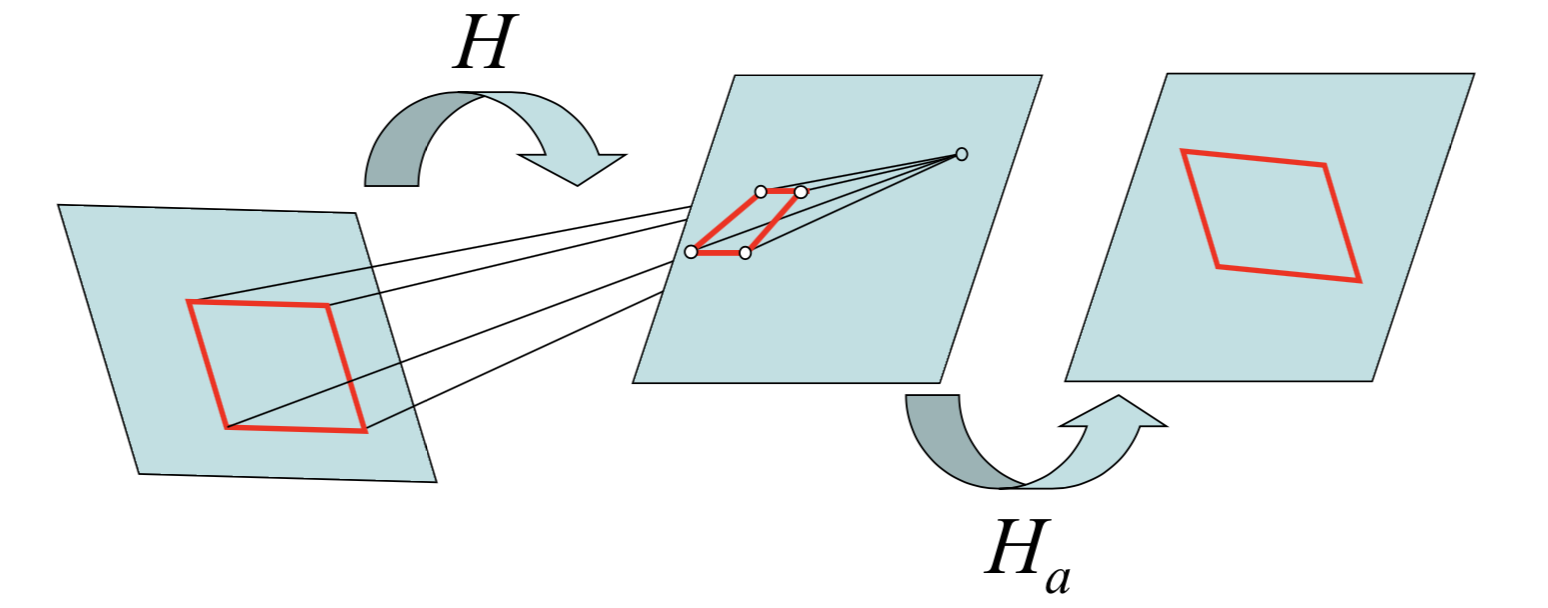
\includegraphics[width=10 cm]{images/affine_rect.png}
\caption{Affine planar rectification}
\label{affine_rect}
\end{center}
\end{figure}
Given a projective version of the world scene, as shown in Fig. \ref{affine_rect}, we may find a homography $H_a$ that preserves the parallelism and thus recovers affine properties as in the original plane. So $H_aH$ is an affine transformation. Actually, $H_a$ can be computed if we know the projection of the line at infinity. In this case, we may denote $l_\infty=\left[\begin{array}{ccc}l_1 & l_2 & l_3\end{array}\right]^\mathsf{T}$. $H_a$ can be expressed as
\begin{align*}
H_a = \left[
\begin{array}{ccc}
1 & 0 & 0 \\
0 & 1 & 0 \\
l_1 & l_2 & l_3
\end{array}\right]
\end{align*}





\section{Metric rectification}
\subsection{For 2D plane}
\begin{figure}[!h]
\begin{center}
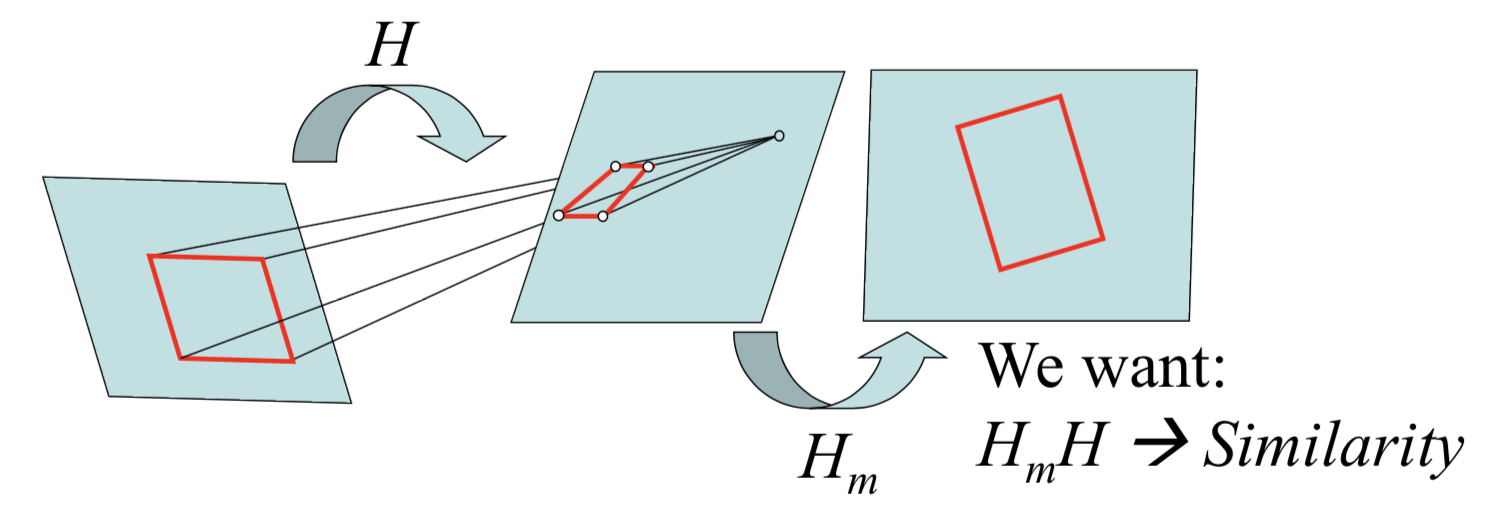
\includegraphics[width=10 cm]{images/metric_rect.png}
\caption{Metric planar rectification}
\label{metric_rect}
\end{center}
\end{figure}
For metric rectification, the euclidean properties of the original plane can be recovered if we find a homography $H_m$, which preserves the angle between two lines on the plane.
We first denote two lines $l=\left[\begin{array}{ccc}a & b & c\end{array}\right]^\mathsf{T}$ and $l'=\left[\begin{array}{ccc}a' & b' & c'\end{array}\right]^\mathsf{T}$. The angle between these two lines is
\begin{align*}
\cos\theta = \frac{aa'+bb'}{\sqrt{a^2+b^2}\sqrt{a'^2+b'^2}}
\end{align*}
Given $aa'+bb'=l'^\mathsf{T} C^\ast l$ and $C^\ast=\left[
      \begin{array}{ccc}
       1 & 0 & 0 \\
       0 & 1 & 0 \\
       0 & 0 & 0 \\
      \end{array}
\right]$, we may derive that
\begin{align*}
\cos\theta = \frac{l'^\mathsf{T} C^\ast l}{\sqrt{l^\mathsf{T} C^\ast l}\sqrt{l'^\mathsf{T} C^\ast l'}}
\end{align*}
If $l'$ and $l$ are orthogonal, we have 
\begin{align*}
l'^\mathsf{T} C^\ast l = 0
\end{align*}

In Fig. \ref{metric_rect}, assume we have a line $l_0$ in the original plane and its homography transformation $l$. After metric rectification, the line became $l'$ and right angle preserved. We get the following equation
\begin{align}
&l'=H^{-\mathsf{T}}_mH^{-\mathsf{T}}l_0=H^{-\mathsf{T}}l \\
&l^{i\mathsf{T}}_0C^\ast l^j_0 = l^{i\mathsf{T}}_0H^{-1}_mC^\ast H^{-\mathsf{T}}_ml^j_0 = 0
\end{align}
To solve for $H_m$, we may need at least 4 pairs of lines.

\subsection{For 3D space}
Assume that we have two perpendicular planes $\pi_1$ and $\pi_2$ in 3D space and $\pi_\infty$ at infinity. $\Omega_\infty$ is an absolute conic on $\pi_\infty$. The dual of the absolute conic $\Omega_\infty$ is called the absolute dual quadric, denoted $\Omega^\ast_\infty$
\begin{align}
\Omega^\ast_\infty = \left[
\begin{array}{cccc}
1 & 0 & 0 & 0 \\
0 & 1 & 0 & 0 \\
0 & 0 & 1 & 0 \\
0 & 0 & 0 & 0 \\
\end{array}\right]
\end{align}
Similarly, the properties are the same as in the plane. The angle between planes is
\begin{align}
\cos\theta = \frac{\pi^\mathsf{T}_1\Omega^\ast_\infty\pi_2}{\sqrt{\pi^\mathsf{T}_1\Omega^\ast_\infty\pi_1}\sqrt{\pi^\mathsf{T}_2\Omega^\ast_\infty\pi_2}}
\end{align}
Note that $C^\ast_\infty$ is invariant if and only if $H$ is a similarity transformation. 


\newpage
\section{Calibration} 
\subsection{Calibration form 3D points (PnP)}
For the camera matrix, $M=K[R\ t]$. We want to solve this intrinsic matrix $K$ from calibration. 
\begin{figure}[H]
\begin{center}
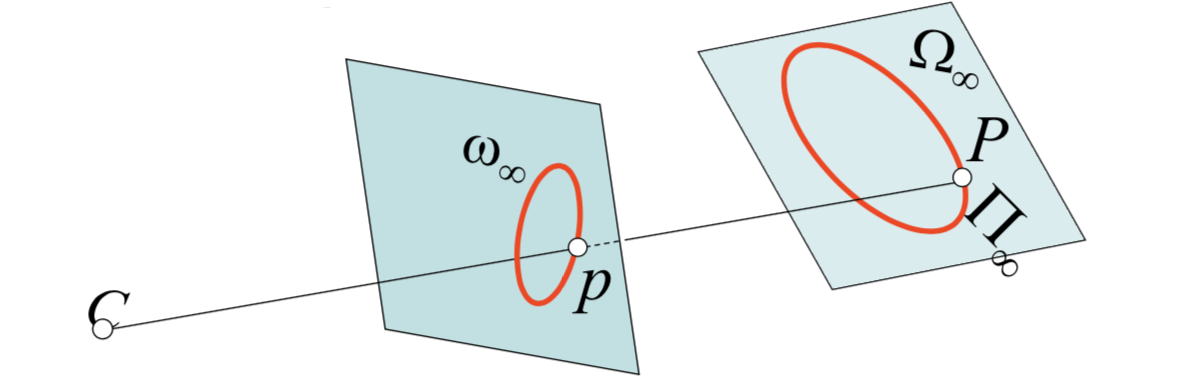
\includegraphics[width=10 cm]{images/calibration.png}
\caption{Calibration from plane homographies: The image of the absolute conic}
\label{calibration}
\end{center}
\end{figure}
Given a plane at infinity $\Pi_\infty$ as in Fig. \ref{calibration}, the absolute conic $\Omega_\infty$ is the conic of equation 
\begin{align}
x^2+y^2+z^2=0, \ w=0
\label{trick1_1}
\end{align}
where $P=\left[\begin{array}{cccc}x & y & z & 0\end{array}\right]^\mathsf{T}$. The point $p$ at the image plane can be expressed as
\begin{align}
&p=k\left[\begin{array}{cc}R & t\end{array}\right]\left[\begin{array}{c}x \\ y \\ z \\ 0\end{array}\right]=KR\left[\begin{array}{c}x \\ y \\ z\end{array}\right] \nonumber\\
&\Longrightarrow \ \left[\begin{array}{c}x \\ y \\ z\end{array}\right]=R^\mathsf{T} K^{-1}p
\label{trick1_2}
\end{align}

From Eqns. \ref{trick1_1} and \ref{trick1_2}, we have
\begin{align}
\left[\begin{array}{ccc}x & y & z\end{array}\right]\left[\begin{array}{c}x \\ y \\ z\end{array}\right]&=0 \nonumber\\
p^\mathsf{T} K^{-\mathsf{T}}RR^\mathsf{T} K^{-1}p&=0 \nonumber\\
p^\mathsf{T} K^{-\mathsf{T}}K^{-1}p&=0 \nonumber\\
p^\mathsf{T} \omega_\infty p&=0
\end{align}
Therefore, $\omega_\infty$ can be represented by the matrix $K^{-\mathsf{T}}K^{-1}$.

\subsection{Outline of the calibration solution}
\begin{figure}[H]
\begin{center}
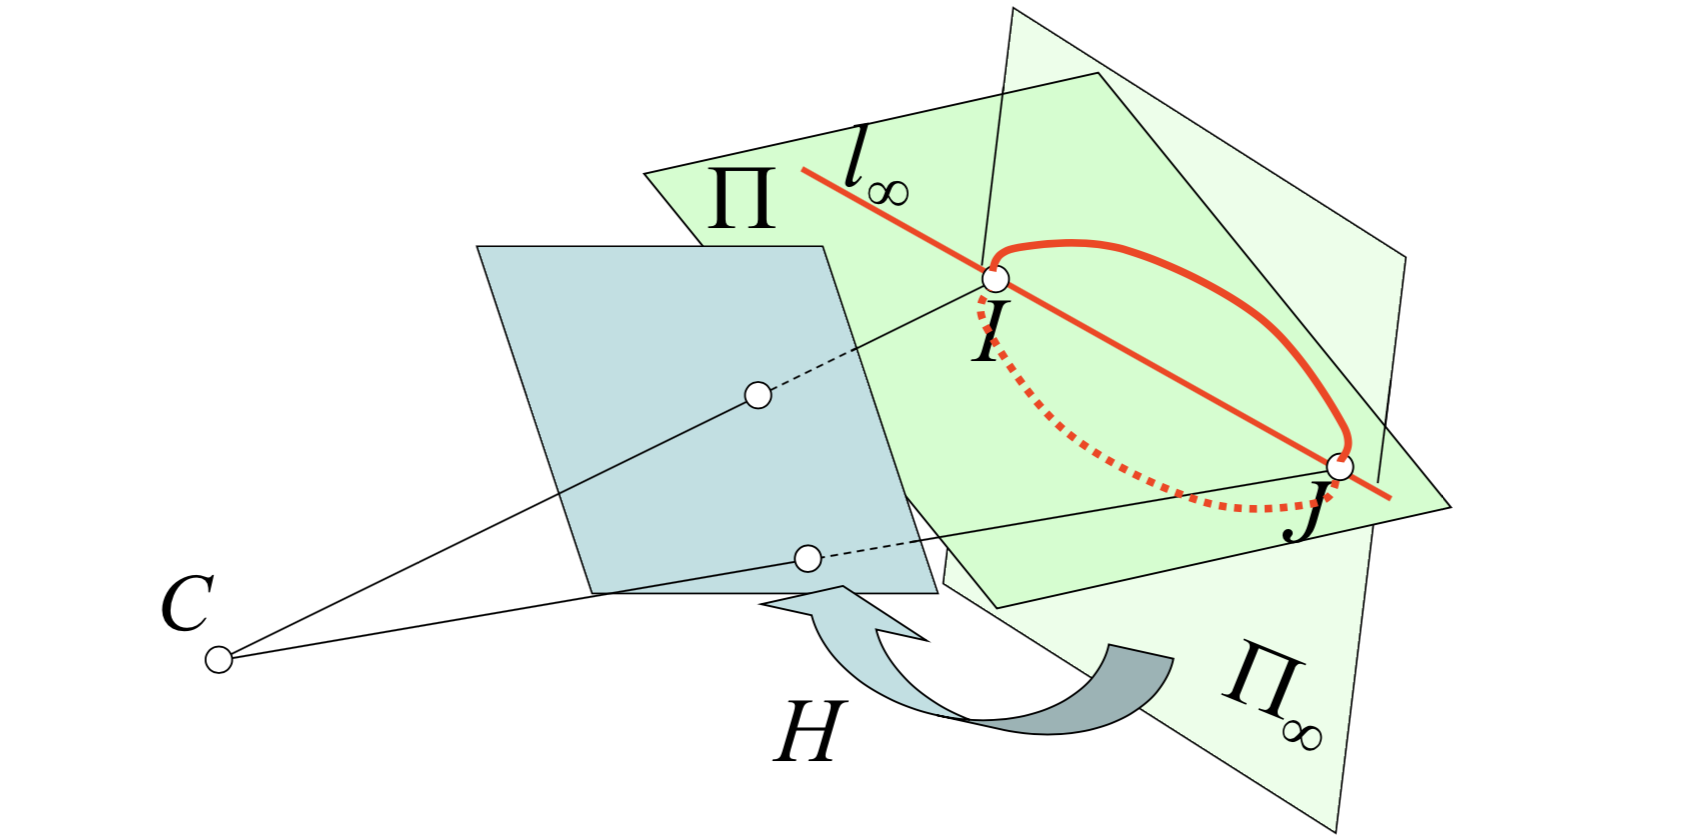
\includegraphics[width=10 cm]{images/plane_at_inf.png}
\caption{Point $I$, $J$ at plane $\Pi_\infty$}
\label{plane_at_inf}
\end{center}
\end{figure}
Now we assume that a plane $\Pi$ intersects the conic $\Omega_\infty$ at point $I,J=\left[\begin{array}{ccc}x & y & 0\end{array}\right]^\mathsf{T}$. Since $x^2+y^2=0$ does not have a real solution. $I$, $J$ can be expressed as 
\begin{align}
I = \left[\begin{array}{c}1 \\ i \\ 0\end{array}\right] \quad J = \left[\begin{array}{c}i \\ -1 \\ 0\end{array}\right]
\end{align}
Since $I\in\Omega_\infty$ and $HI\in\omega_\infty$, we know
\begin{align*}
I^\mathsf{T} H^\mathsf{T}\omega_\infty HI=0\\
J^\mathsf{T} H^\mathsf{T}\omega_\infty HI=0
\end{align*}
Thus we have 2 equations per plane. Note that $\omega_\infty$ has 5 dof since a $3\times3$ matrix gives 6 dof while it is also up to scale. 


\section{PnP solutions}
Suppose we have 3 world coordinates of point $i$: $p^w_i=\left[\begin{array}{ccc}x^w_i & y^w_i & z^w_i\end{array}\right]^\mathsf{T}$, and 3 coordinates of point $i$ with respect to camera coordinate system: $p^c_i=\left[\begin{array}{ccc}x^c_i & y^c_i & z^c_i\end{array}\right]^\mathsf{T}$. 

Now let $M=K\left[\begin{array}{cc}R & t\end{array}\right]$, in this case $K$ is a known variable. Since we have $p=MP$, $M=\left[\begin{array}{c}\textbf{m}^\mathsf{T}_1\\\textbf{m}^\mathsf{T}_2\\\textbf{m}^\mathsf{T}_3\end{array}\right]$,
\begin{align*}
& x=\frac{\textbf{m}^\ttt_1P}{\textbf{m}^\ttt_3P}, \quad y=\frac{\textbf{m}^\ttt_2P}{\textbf{m}^\ttt_3P}
\end{align*}
\begin{align}
\Rightarrow & \ \left\{
\begin{array}{l}
P^\ttt_i\textbf{m}_1-xP^\ttt_i\textbf{m}_3=0 \\
P^\ttt_i\textbf{m}_2-yP^\ttt_i\textbf{m}_3=0
\end{array}\right.
\label{dlt_raw}
\end{align}
Suppose we have $N$ sets of Eqn. \ref{dlt_raw}, we may write in the matrix form
\begin{align}
\left[\begin{array}{ccc}
P^\ttt_i & 0 & -xP^\ttt_i \\
0 & P^\ttt_i & -yP^\ttt_i \\
 & \vdots & 
\end{array}\right]
\left[\begin{array}{c}
\textbf{m}_1 \\
\textbf{m}_2 \\
\textbf{m}_3
\end{array}\right]=0
\end{align}





\end{document}
